% =========================================================================
% CHAPTER 2: CƠ SỞ LÝ THUYẾT
% =========================================================================

\section{Cơ sở lý thuyết}

% --- SLIDE 2.1: Campus Network ---
\begin{frame}{2.1 Campus Network và kiến trúc phân cấp}
    \begin{columns}[T]
        \column{0.48\textwidth}
        \textbf{Campus Network} là mạng kết nối người dùng, thiết bị và dịch vụ trong một khuôn viên hoặc một tổ chức.
        \vspace{0.2cm}
        \begin{itemize}
            \item Phục vụ số lượng lớn thiết bị đầu cuối.
            \item Phân chia người dùng theo đơn vị và chức năng.
            \item Yêu cầu khả năng quản lý, dự phòng và bảo mật.
        \end{itemize}

        \column{0.48\textwidth}
        \textbf{Mô hình ba lớp:}
        \begin{itemize}
            \item \textbf{Core:} chuyển tiếp tốc độ cao, kết nối các khối chính.
            \item \textbf{Distribution:} tổng hợp truy cập, định tuyến và áp dụng chính sách.
            \item \textbf{Access:} kết nối thiết bị người dùng và gán VLAN.
        \end{itemize}
    \end{columns}
    \vspace{0.15cm}
    \begin{block}{Ý nghĩa của phân tầng}
        Tách rõ chức năng giúp kiến trúc dễ quản lý, dễ xác định phạm vi sự cố và thuận lợi khi thay đổi quy mô.
    \end{block}
\end{frame}

% --- SLIDE 2.2: SDN ---
\begin{frame}{2.2 Software-Defined Networking (SDN)}
    \begin{columns}[T]
        \column{0.48\textwidth}
        \textbf{Nguyên lý cốt lõi:}
        \begin{itemize}
            \item Tách \textbf{Control Plane} khỏi \textbf{Data Plane}.
            \item Controller duy trì góc nhìn logic tập trung về hệ thống.
            \item Thiết bị chuyển tiếp thực thi các flow rule do Controller cung cấp.
        \end{itemize}

        \column{0.48\textwidth}
        \textbf{Các lớp chức năng:}
        \begin{itemize}
            \item \textbf{Application Layer:} biểu diễn chính sách và ứng dụng mạng.
            \item \textbf{Control Layer:} tính toán và phân phối quyết định điều khiển.
            \item \textbf{Infrastructure Layer:} chuyển tiếp lưu lượng thực tế.
        \end{itemize}
    \end{columns}
    \vspace{0.15cm}
    \begin{block}{Giao diện tiêu biểu}
        Northbound API kết nối ứng dụng với Controller; \textbf{OpenFlow} là một giao thức Southbound giữa Controller và switch.
    \end{block}
\end{frame}

% --- SLIDE 2.2.1: Hình minh họa kiến trúc SDN ---
\begin{frame}{2.2.1 Kiến trúc phân lớp của SDN}
    \centering
    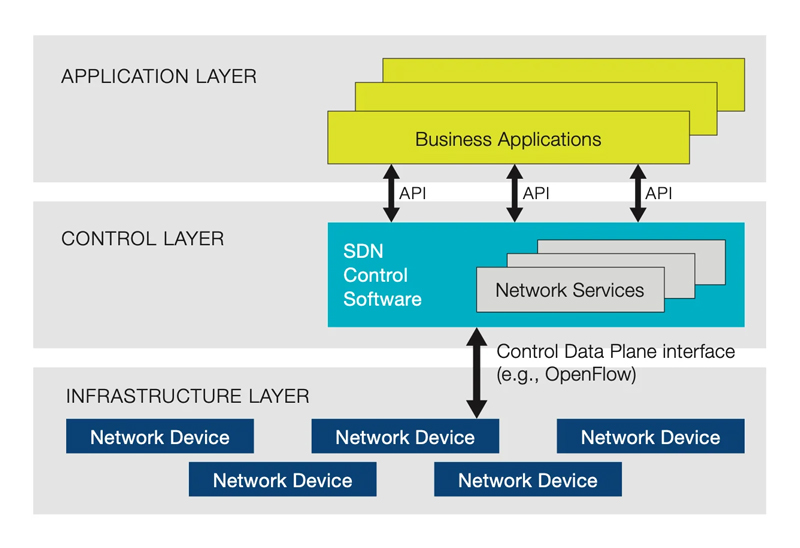
\includegraphics[
        width=0.9\textwidth,
        height=0.72\textheight,
        keepaspectratio
    ]{images/kien-truc-cua-software-defined-networking.jpg}

    \vspace{0.1cm}
    {\scriptsize\textit{Hình 2.1: Ba lớp chức năng trong kiến trúc Software-Defined Networking}}
\end{frame}

% --- SLIDE 2.3: SD-WAN ---
\begin{frame}{2.3 Software-Defined WAN (SD-WAN)}
    \begin{columns}[T]
        \column{0.48\textwidth}
        \textbf{Hai lớp mạng chính:}
        \begin{itemize}
            \item \textbf{Underlay:} hạ tầng truyền dẫn sẵn có như Internet hoặc MPLS.
            \item \textbf{Overlay:} mạng logic hình thành giữa các WAN Edge.
            \item Tunnel bảo mật vận chuyển dữ liệu giữa các site.
        \end{itemize}

        \column{0.48\textwidth}
        \textbf{Các vai trò điều khiển:}
        \begin{itemize}
            \item Quản lý tập trung và cung cấp thông tin vận hành.
            \item Điều phối việc tham gia overlay của thiết bị biên.
            \item Phân phối thông tin định tuyến và chính sách giữa các site.
        \end{itemize}
    \end{columns}
    \vspace{0.15cm}
    \begin{block}{Đặc trưng kiến trúc}
        Lớp overlay độc lập tương đối với hạ tầng truyền dẫn, nhờ đó có thể sử dụng nhiều loại đường WAN trong cùng một mô hình.
    \end{block}
\end{frame}

% --- SLIDE 2.4: So sánh vai trò ---
\begin{frame}{2.4 Vai trò của SDN và SD-WAN trong đề tài}
    \begin{table}
        \centering
        \small
        \renewcommand{\arraystretch}{1.35}
        \begin{tabular}{|p{0.2\textwidth}|p{0.35\textwidth}|p{0.35\textwidth}|}
            \hline
            \rowcolor{primaryDark!15}
            \textbf{Tiêu chí} & \textbf{SDN} & \textbf{SD-WAN} \\
            \hline
            Phạm vi & Mạng nội bộ trong Campus & Kết nối WAN giữa các cơ sở \\
            \hline
            Đối tượng & Switch và luồng dữ liệu nội bộ & WAN Edge, tunnel và route overlay \\
            \hline
            Trọng tâm & Điều khiển tập trung, chính sách luồng & Điều phối kết nối đa đường truyền \\
            \hline
            Giao thức tiêu biểu & OpenFlow & OMP, IPsec \\
            \hline
            Vai trò chung & \multicolumn{2}{c|}{Tách logic điều khiển khỏi hạ tầng chuyển tiếp} \\
            \hline
        \end{tabular}
    \end{table}
\end{frame}

% --- SLIDE 2.5: Nền tảng giao thức ---
\begin{frame}{2.5 Các giao thức và cơ chế nền tảng}
    \begin{columns}[T]
        \column{0.48\textwidth}
        \textbf{Trong Campus:}
        \begin{itemize}
            \item \textbf{VLAN/802.1Q:} phân tách miền quảng bá.
            \item \textbf{OSPF:} trao đổi thông tin định tuyến nội bộ.
            \item \textbf{VRRP:} cung cấp gateway logic dự phòng.
            \item \textbf{DHCP:} cấp phát tham số mạng cho đầu cuối.
        \end{itemize}

        \column{0.48\textwidth}
        \textbf{Trong SDN và SD-WAN:}
        \begin{itemize}
            \item \textbf{OpenFlow:} quản lý bảng flow trên switch.
            \item \textbf{OMP:} trao đổi route và thông tin overlay.
            \item \textbf{IPsec:} bảo vệ dữ liệu qua đường WAN.
            \item \textbf{ACL/Firewall:} kiểm soát truy cập giữa các vùng.
        \end{itemize}
    \end{columns}
\end{frame}
